\documentclass[a4paper,12pt,twoside,final,spanish]{article}
%titlepage: pone el título en una página aparte
%twocolumn
\usepackage{babel} %Para el lenguaje [spanish]
\usepackage[utf8]{inputenc} %Para reconocer todos los símbolos
\usepackage[T1]{fontenc}
\usepackage{textcomp}
\usepackage{amsmath}
\usepackage{amsfonts}
\usepackage{amssymb}
\usepackage[margin=2cm]{geometry} %Márgenes
\usepackage[T1]{fontenc}
\usepackage{graphicx}
\usepackage{enumerate}
\usepackage{hyperref}
\pagestyle{headings}
%---
\usepackage{geometry}
\geometry{text={7in,9.5in},headheight=15pt}
%\textwidth = 7 in
%\textheight = 9.5 in
%\oddsidemargin = -0.25 in
%\evensidemargin = 0.0 in
%\topmargin = -0.25 in
%\headheight = 0.0 in
%\headsep = 0.0 in
\setlength{\parskip}{0.1in}
\setlength{\parindent}{0.0in}
%---
\usepackage{fancyhdr} %Para usar encabezados y pies personalizados
	\pagestyle{fancy}
	\fancyhf{}
	\fancyhead[LE,RO]{Tecnologías para la Web Semántica} 
	\fancyhead[RE,LO]{Arquitectura}
	\fancyfoot[RE,LO]{Darién Julián Ramírez}
	\fancyfoot[LE,RO]{\thepage}
	\renewcommand{\footrulewidth}{1pt}
%---
\usepackage{listings} %Para escribir códigos
\lstset{language=XML,
	basicstyle=\footnotesize,
	numbers=left,
 	stepnumber=1,
	numbersep=8pt,
	showspaces=false,               % show spaces adding particular underscores
  	showstringspaces=false,         % underline spaces within strings
  	frame=lines,                   % adds a frame around the code
	tabsize=4,                      
  	captionpos=b,                   % sets the caption-position to bottom
  	breaklines=true,                % sets automatic line breaking
}
%---

\title{\Huge Tecnologías para la Web Semántica\\
Trabajo Práctico Nº5\\
Arquitectura}
\author{Darién Julián Ramírez}
\date{\vspace{-5ex}}

\begin{document}

\maketitle %Crea la página de título

\section*{Ejercicio 1}

Defina en XML la siguiente orden de compra:

\begin{center}
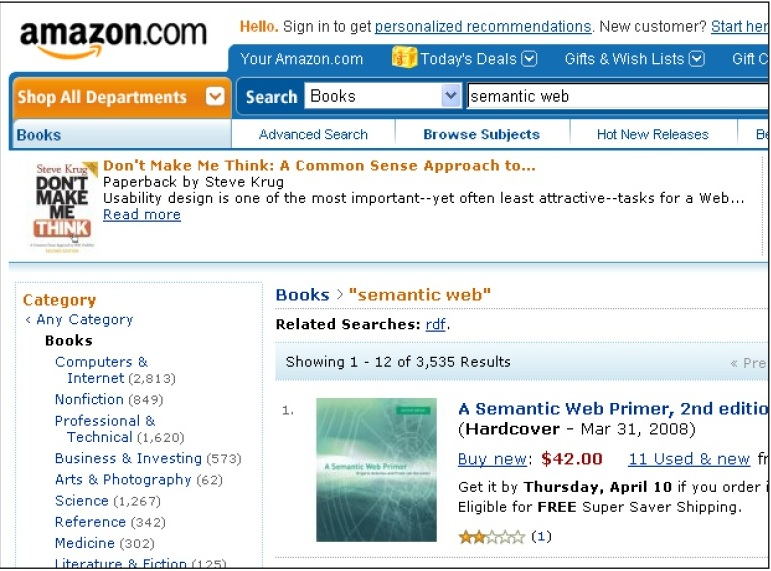
\includegraphics[width=0.9\linewidth,keepaspectratio]{1}
\end{center}

\begin{center}
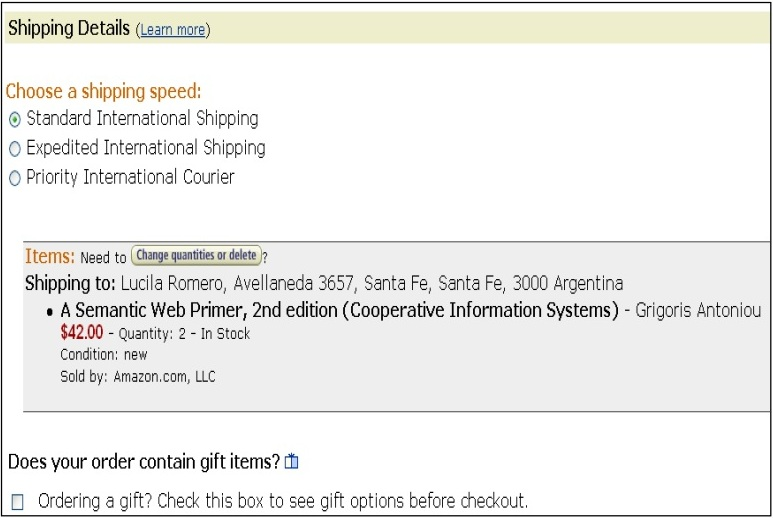
\includegraphics[width=0.9\linewidth,keepaspectratio]{2}
\end{center}

\dotfill

\begin{lstlisting}
<orden_de_compra>
 <libro>
 	<titulo> A semantic web primer </titulo>
 	<edicion> segunda </edicion>
 	<precio> $42 </precio>
 	<estado> nuevo </estado>
 	<fecha_de_publicacion> 2008 </fecha_de_publicacion>
 </libro>
 <tiempo_de_envio> estandar </tiempo_de_envio>
 <destinatario>
 	<nombre> Lucila Romero </nombre>
 	<direccion> Avellaneda 3657 </direccion>
 	<pais> argentina </pais>
 	<provincia> santa fe </provincia>
 	<ciudad> santa fe </ciudad>
 	<cp> 3000 </cp>
 </destinatario>
<orden_de_compra>
\end{lstlisting}

\section*{Ejercicio 2}

Defina en XML los datos correspondientes al siguiente sitio: 

\begin{center}
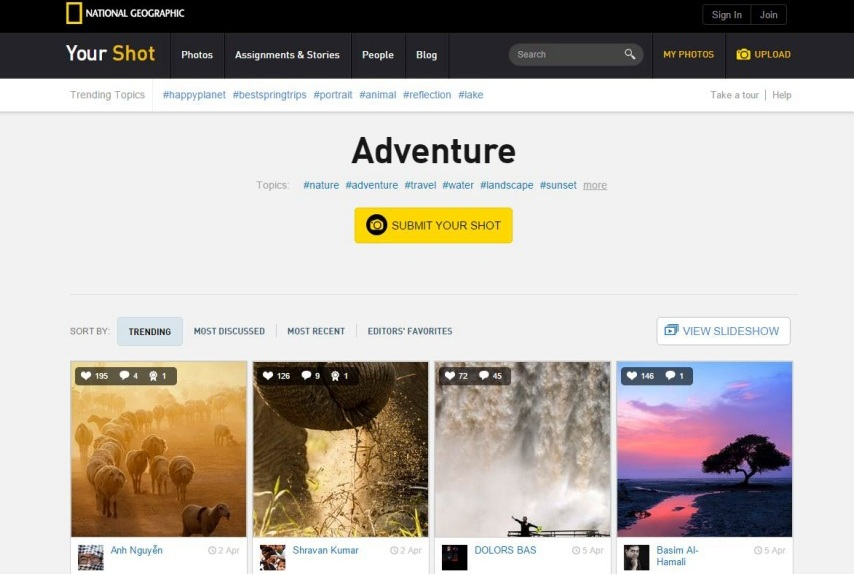
\includegraphics[width=0.9\linewidth,keepaspectratio]{3}
\end{center}

\dotfill

\begin{lstlisting}
<natgeo>
	<webpage>
		<your_shot>
		 <ordenado_por> trending </ordenado_por>
		 <foto>
		 	<autor> Anh Nguyen </autor>
		 	<vistas> 195 </vistas>
		 	<comentarios> 4 </comentarios>
		 	<likes> 1 </likes>
		 </foto>
		 <foto>
		 	<autor> Shavan Kumar </autor>
		 	<vistas> 126 </vistas>
		 	<comentarios> 9 </comentarios>
		 	<likes> 1 </likes>
		 </foto>
		 <foto>
		 	<autor> DOLORS BAS </autor>
		 	<vistas> 72 </vistas>
		 	<comentarios> 45 </comentarios>
		 	<likes> 0 </likes>
		 </foto>
		 <foto>
		 	<autor> Basin Al-Hamali </autor>
		 	<vistas> 145 </vistas>
		 	<comentarios> 1 </comentarios>
		 	<likes> 0 </likes>
		 </foto>
		</your_shot>
	</webpage>
</natgeo>
\end{lstlisting}

\section*{Ejercicio 3}

Redefina los elementos XML de manera tal de reemplazar atributos por elementos anidados:

\begin{lstlisting}
<order order No="23456" customer="John Smith" date="October 15, 2002"> 
  <item itemNo="c817" quantity="1"/> 
  <item itemNo="a528" quantity="3"/> 
</order>
\end{lstlisting}

\dotfill

\begin{lstlisting}
<orden_de_compra libro="A semantic web primer" edicion="segunda" precio="$42" estado="nuevo" fecha_de_publicacion="2008"> 
	<tiempo_de_envio="estandar">
	<destinatario nombre="Lucila Romero" direccion="Avellaneda 3657" pais="argentina" provincia="santa fe" ciudad="santa fe" cp="3000">
</orden_de_compra>
\end{lstlisting}

\section*{Ejercicio 4}

¿Qué es una red semántica? Defina, explique y ejemplifique.

\dotfill

Una red semántica o esquema de representación en Red es una forma de representación de conocimiento lingüístico en la que los conceptos y sus interrelaciones se representan mediante un grafo. En caso de que no existan ciclos, estas redes pueden ser visualizadas como árboles. Las redes semánticas son usadas, entre otras cosas, para representar mapas conceptuales y mentales.

En un grafo o red semántica los elementos semánticos se representan por nodos. Dos elementos semánticos entre los que se admite se da la relación semántica que representa la red, estarán unidos mediante una línea, flecha o enlace o arista. Cierto tipo de relaciones no simétricas requieren grafos dirigidos que usan flechas en lugar de líneas.

\begin{center}
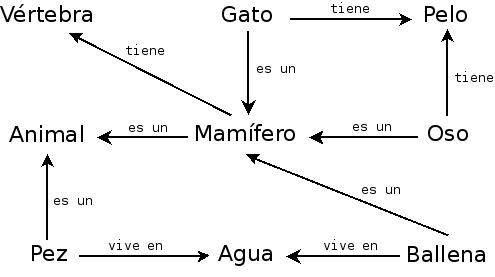
\includegraphics[width=0.9\linewidth,keepaspectratio]{5.png}
\end{center}

Existen diversos tipos de relaciones semánticas como la hiponimia, hiperonimia, la meronimia, etc. Dado un conjunto de conceptos, elementos semánticos o términos relacionados semánticamente mediante alguna relación semántica, una red semántica representa estas relaciones en forma de grafo. Explícitamente, dado un conjunto de términos {t1, t2,..., tn} y cierta relación semántica simétrica entre ellos se construye un grafo G = (V,A) cumpliendo las siguientes condiciones:
\begin{enumerate}[a.]
\item El conjunto V es el conjunto de vértices o nodos del grafo. Este conjunto estará formado por n elementos (tantos vértices como términos relacionables). A cada uno de los vértices del grafo representará uno de los términos, por tanto los vértices del grafo se llamarán: t1, t2,..., tn.
\item El conjunto A es el conjunto de aristas o líneas del grafo. Dados dos vértices (términos) del grafo ti y tj existirá una línea aij que une los vértices ti y tj si y sólo si los términos de pona ti y tj están relacionados.
\end{enumerate}

Si la relación no es simétrica, entonces se usan grafos dirigidos para representar la relación.

\section*{Ejercicio 5}

Dados los casos detallados más abajo:

\begin{enumerate}[a.]
\item Identifique las tripletas Sujeto-Predicado-Objeto.

\dotfill

\begin{lstlisting}
Caso 1:

http://www.w3.org/RDF/Validator/run/1493053369633#spiderman
http://www.w3.org/1999/02/22-rdf-syntax-ns#type
http://xmlns.com/foaf/0.1/Person

http://www.w3.org/RDF/Validator/run/1493053369633#spiderman
http://xmlns.com/foaf/0.1/name
"Spiderman"

http://www.w3.org/RDF/Validator/run/1493053369633#spiderman
http://www.perceive.net/schemas/relationship/enemyOf
http://www.w3.org/RDF/Validator/run/1493053369633#green-goblin

http://www.w3.org/RDF/Validator/run/1493053369633#green-goblin
http://www.w3.org/1999/02/22-rdf-syntax-ns#type
http://xmlns.com/foaf/0.1/Person

http://www.w3.org/RDF/Validator/run/1493053369633#green-goblin
http://xmlns.com/foaf/0.1/name
"Green Goblin"

http://www.w3.org/RDF/Validator/run/1493053369633#green-goblin
http://www.perceive.net/schemas/relationship/enemyOf
http://www.w3.org/RDF/Validator/run/1493053369633#spiderman

http://www.w3.org/RDF/Validator/run/1493053369633#peter
http://www.w3.org/1999/02/22-rdf-syntax-ns#type
http://xmlns.com/foaf/0.1/Person

http://www.w3.org/RDF/Validator/run/1493053369633#peter
http://xmlns.com/foaf/0.1/name
"Peter Parker"

http://www.w3.org/RDF/Validator/run/1493053369633#peter
http://www.perceive.net/schemas/relationship/friendOf
http://www.w3.org/RDF/Validator/run/1493053369633#harry

http://www.w3.org/RDF/Validator/run/1493053369633#harry
http://www.w3.org/1999/02/22-rdf-syntax-ns#type
http://xmlns.com/foaf/0.1/Person

http://www.w3.org/RDF/Validator/run/1493053369633#harry
http://xmlns.com/foaf/0.1/name
"Harry Osborn"

http://www.w3.org/RDF/Validator/run/1493053369633#harry
http://www.perceive.net/schemas/relationship/friendOf
http://www.w3.org/RDF/Validator/run/1493053369633#peter

http://www.w3.org/RDF/Validator/run/1493053369633#harry
http://www.perceive.net/schemas/relationship/childOf
http://www.w3.org/RDF/Validator/run/1493053369633#norman

http://www.w3.org/RDF/Validator/run/1493053369633#norman
http://www.w3.org/1999/02/22-rdf-syntax-ns#type
http://xmlns.com/foaf/0.1/Person

http://www.w3.org/RDF/Validator/run/1493053369633#norman
http://xmlns.com/foaf/0.1/name
"Norman Osborn"

http://www.w3.org/RDF/Validator/run/1493053369633#norman
http://www.perceive.net/schemas/relationship/parentOf
http://www.w3.org/RDF/Validator/run/1493053369633#harry
\end{lstlisting}

\begin{lstlisting}
Caso 2:

http://qqqfoo.com/staff/corky
http://www.w3.org/2001/vcard-rdf/3.0#FN
"Corky Crystal"

http://qqqfoo.com/staff/corky
http://www.w3.org/2001/vcard-rdf/3.0#N
genid:A7264

genid:A7264
http://www.w3.org/2001/vcard-rdf/3.0#Family
"Crystal"

genid:A7264
http://www.w3.org/2001/vcard-rdf/3.0#Given
"Corky"

genid:A7264
http://www.w3.org/2001/vcard-rdf/3.0#Other
"Jacky"

genid:A7264
http://www.w3.org/2001/vcard-rdf/3.0#Prefix
"Dr"

http://qqqfoo.com/staff/corky
http://www.w3.org/2001/vcard-rdf/3.0#BDAY
"1980-01-01"

http://qqqfoo.com/staff/corky
http://www.w3.org/2001/vcard-rdf/3.0#TITLE
"Computer Officer Class 3"

http://qqqfoo.com/staff/corky
http://www.w3.org/2001/vcard-rdf/3.0#ROLE
"Programmer"

http://qqqfoo.com/staff/corky
http://www.w3.org/2001/vcard-rdf/3.0#TEL
genid:A7265

genid:A7265
http://www.w3.org/1999/02/22-rdf-syntax-ns#value
"+61 7 555 5555"

genid:A7265
http://www.w3.org/1999/02/22-rdf-syntax-ns#type
http://www.w3.org/2001/vcard-rdf/3.0#work

genid:A7265
http://www.w3.org/1999/02/22-rdf-syntax-ns#type
http://www.w3.org/2001/vcard-rdf/3.0#voice

http://qqqfoo.com/staff/corky
http://www.w3.org/2001/vcard-rdf/3.0#EMAIL
genid:A7266

genid:A7266
http://www.w3.org/1999/02/22-rdf-syntax-ns#value
"corky@qqqfoo.com"

genid:A7266
http://www.w3.org/1999/02/22-rdf-syntax-ns#type
http://www.w3.org/2001/vcard-rdf/3.0#internet

http://qqqfoo.com/staff/corky
http://www.w3.org/2001/vcard-rdf/3.0#ADR
genid:A7267

genid:A7267
http://www.w3.org/2001/vcard-rdf/3.0#Street
"111 Lake Drive"

genid:A7267
http://www.w3.org/2001/vcard-rdf/3.0#Locality
"WonderCity"

genid:A7267
http://www.w3.org/2001/vcard-rdf/3.0#Pcode
"5555"

genid:A7267
http://www.w3.org/2001/vcard-rdf/3.0#Country
"Australia"
\end{lstlisting}

\item Obtenga el grafo o red semántica correspondiente.

\dotfill

\begin{center}
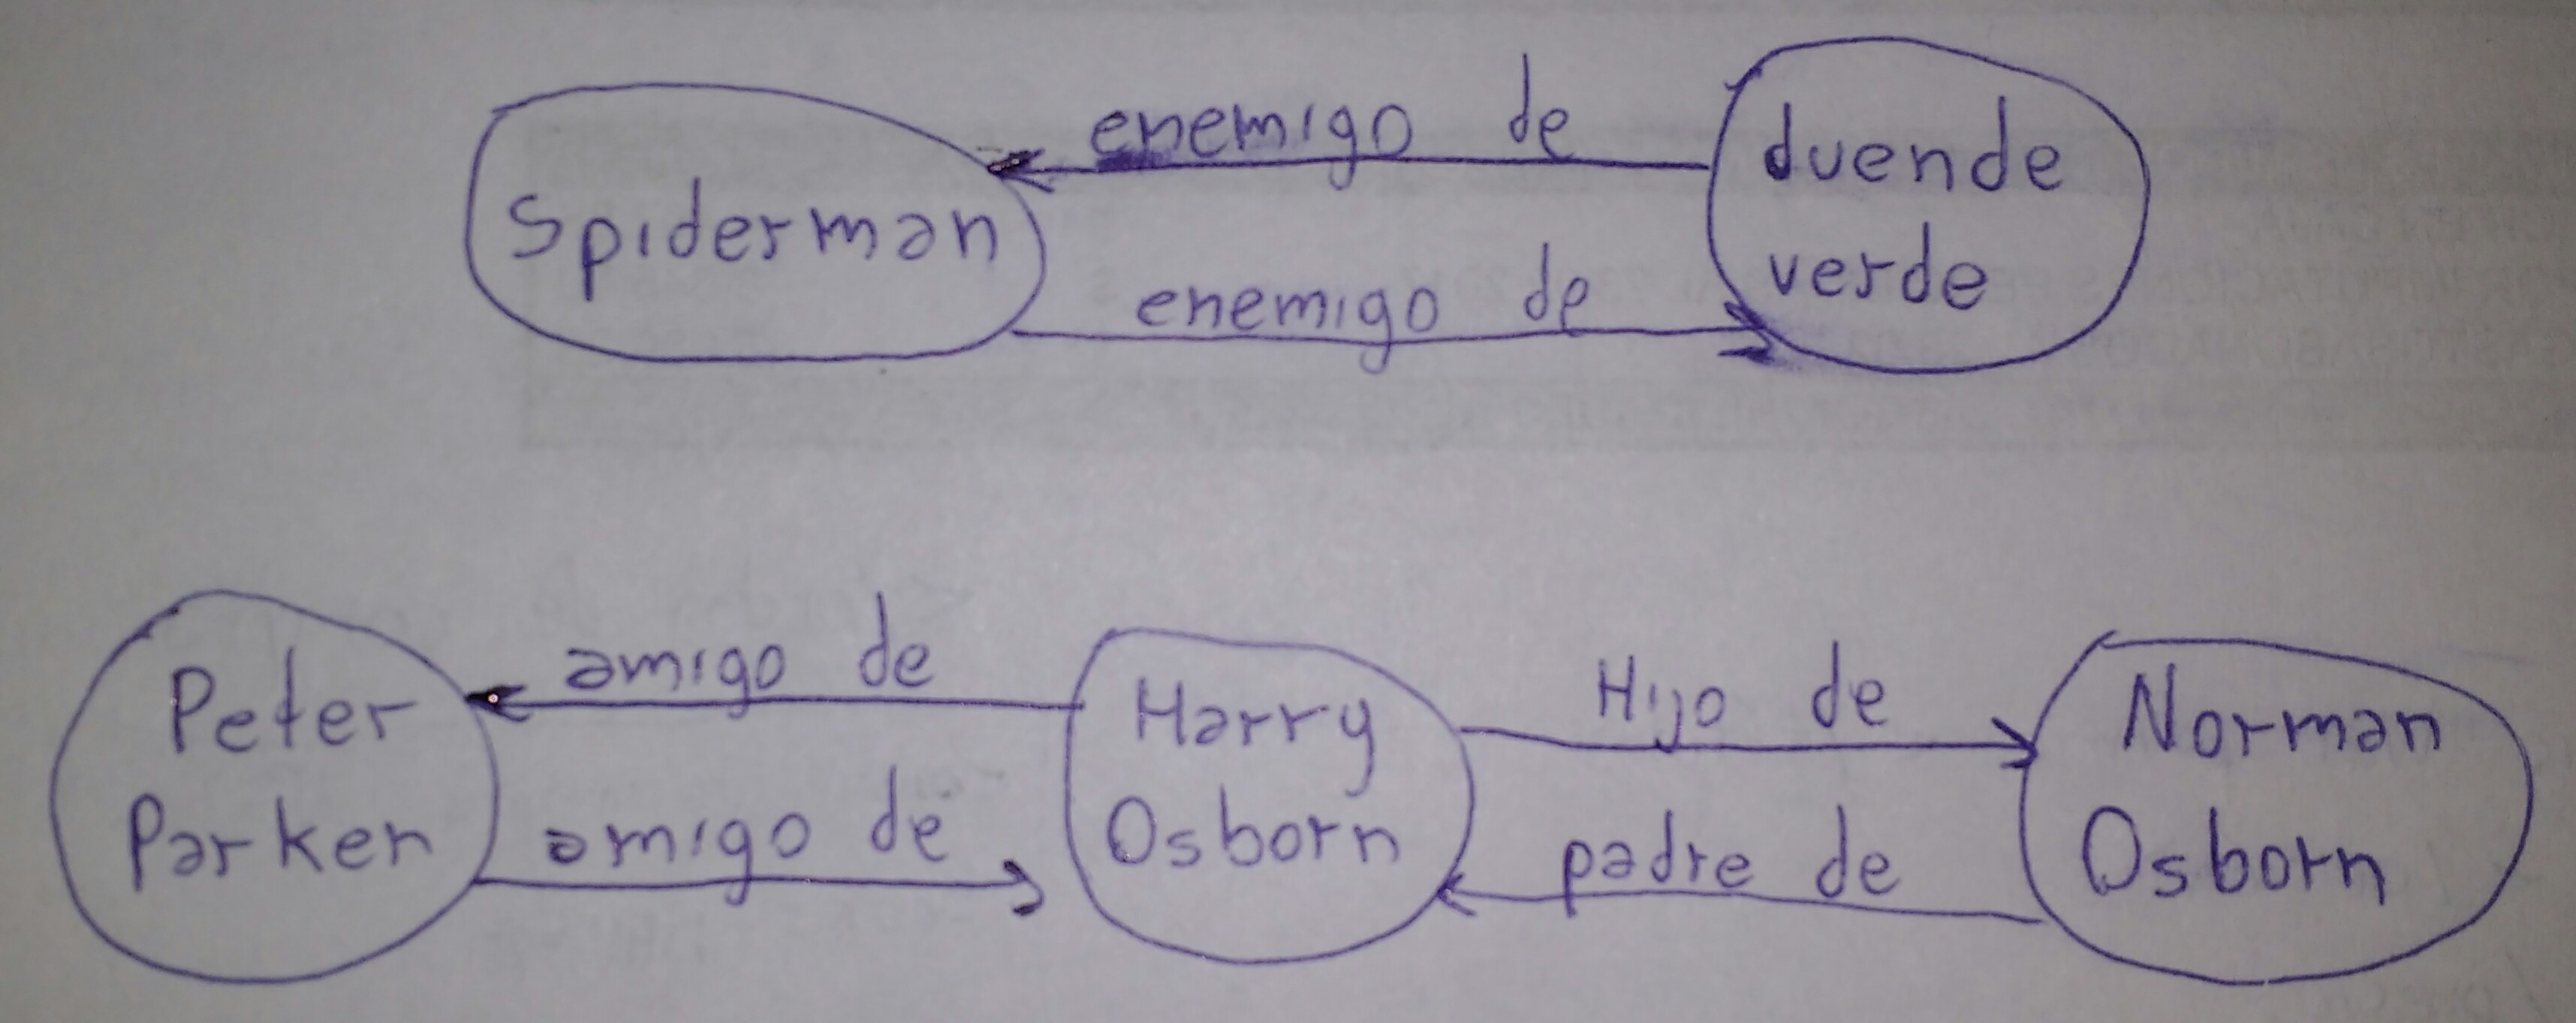
\includegraphics[width=0.9\linewidth,keepaspectratio]{4.jpg}
\end{center}

\item ¿A qué formato estándar corresponde el prefijo vCard? ¿Para qué se utiliza?

\dotfill

\begin{quote}
vCard es un formato estándar para el intercambio de información personal, específicamente tarjetas personales electrónicas (electronic business cards). Las vCards son usualmente adjuntadas a mensajes de correo electrónico, pero pueden ser intercambiadas en muchas otras formas, como en la World Wide Web o a través de códigos QR. Pueden contener nombre, dirección, números telefónicos, URLs, logos, fotografías, e incluso clips de audio.
\end{quote}

\end{enumerate}

\textbf{Nota:} Es posible utilizar el parser RDF para validar las sentencias.\\
\url{http://www.w3.org/RDF/Validator}

\textbf{Caso 1:}
\begin{lstlisting}
<rdf:RDF xmlns:rdf="http://www.w3.org/1999/02/22-rdf-syntax-ns#"
         xmlns:foaf="http://xmlns.com/foaf/0.1/"
         xmlns:rel="http://www.perceive.net/schemas/relationship/">
         
<foaf:Person rdf:ID="spiderman">
	<foaf:name>Spiderman</foaf:name>   
   	<rel:enemyOf rdf:resource="#green-goblin"/>
</foaf:Person>

<foaf:Person rdf:ID="green-goblin">
	<foaf:name>Green Goblin</foaf:name>
   	<rel:enemyOf rdf:resource="#spiderman"/>
</foaf:Person> 

<foaf:Person rdf:ID="peter">
	<foaf:name>Peter Parker</foaf:name>
   	<rel:friendOf rdf:resource="#harry"/>
</foaf:Person>

<foaf:Person rdf:ID="harry">
	<foaf:name>Harry Osborn</foaf:name>
   	<rel:friendOf rdf:resource="#peter"/>
   	<rel:childOf rdf:resource="#norman"/>
</foaf:Person>

<foaf:Person rdf:ID="norman">
 	<foaf:name>Norman Osborn</foaf:name>
   	<rel:parentOf rdf:resource="#harry"/>   
</foaf:Person>
 
</rdf:RDF>
\end{lstlisting}

\textbf{Caso 2:}
\begin{lstlisting}
<?xml version="1.0"?> 
<rdf:RDF xmlns:rdf = "http://www.w3.org/1999/02/22-rdf-syntax-ns#" 
xmlns:vCard = "http://www.w3.org/2001/vcard-rdf/3.0#">  
<rdf:Description rdf:about = "http://qqqfoo.com/staff/corky" > 
<vCard:FN> Corky Crystal </vCard:FN> 
<vCard:N rdf:parseType="Resource"> 
<vCard:Family> Crystal </vCard:Family> 
<vCard:Given> Corky </vCard:Given> 
<vCard:Other> Jacky </vCard:Other> 
<vCard:Prefix> Dr </vCard:Prefix> 
</vCard:N> 
<vCard:BDAY> 1980-01-01 </vCard:BDAY> 
<vCard:TITLE> Computer Officer Class 3 </vCard:TITLE> 
<vCard:ROLE> Programmer </vCard:ROLE> 
<vCard:TEL rdf:parseType="Resource"> 
<rdf:value> +61 7 555 5555 </rdf:value> 
<rdf:type rdf:resource="http://www.w3.org/2001/vcard-rdf/3.0#work"/> 
<rdf:type rdf:resource="http://www.w3.org/2001/vcard-rdf/3.0#voice"/> 
</vCard:TEL> 
<vCard:EMAIL rdf:parseType="Resource"> 
<rdf:value> corky@qqqfoo.com </rdf:value> 
<rdf:type rdf:resource="http://www.w3.org/2001/vcard-rdf/3.0#internet"/> 
</vCard:EMAIL> 
<vCard:ADR rdf:parseType="Resource"> 
<vCard:Street> 111 Lake Drive </vCard:Street> 
<vCard:Locality> WonderCity </vCard:Locality> 
<vCard:Pcode> 5555 </vCard:Pcode> 
<vCard:Country> Australia </vCard:Country> 
</vCard:ADR> 
</rdf:Description> 
</rdf:RDF> 
\end{lstlisting}

\section*{Ejercicio 6}

Utilice el generador de ficheros RDF para describir fotografías e imágenes.\\
\url{http://webposible.com/utilidades/generador_rdf_foto.html}

\begin{enumerate}[a.]
\item Seleccione una imagen de la web y descríbala según los pasos solicitados en el generador. 

\dotfill

\begin{center}
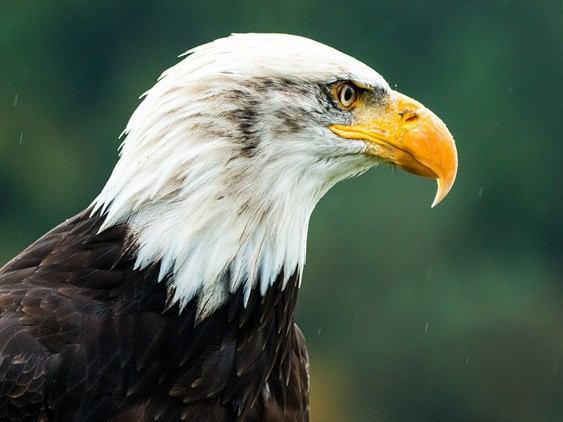
\includegraphics[width=0.9\linewidth,keepaspectratio]{6.jpg}
\end{center}

\begin{lstlisting}
<?xml version="1.0" encoding="utf-8"?>
<rdf:RDF xmlns:dc="http://purl.org/dc/elements/1.1/"
	xmlns:h="http://www.w3.org/1999/xhtml"
	xmlns:hr="http://www.w3.org/2000/08/w3c-synd/#"
	xmlns:rdf="http://www.w3.org/1999/02/22-rdf-syntax-ns#"
	xmlns:rdfs="http://www.w3.org/2000/01/rdf-schema#"
	xmlns:s1="http://www.w3.org/2000/PhotoRDF/technical-1-0#"
	xmlns:tiff="http://ns.adobe.com/tiff/1.0/"
	xmlns:exif="http://ns.adobe.com/exif/1.0/"
	xmlns:photoshop="http://ns.adobe.com/photoshop/1.0/"
	xmlns:xmpRights="http://ns.adobe.com/xap/1.0/rights/"
	xmlns:NewsML="http://www.iptc.org/NewsML/1.0/specification/NewsML_1.0.dtd"
	xmlns:admin="http://webns.net/mvcb/"
	xmlns:foaf="http://xmlns.com/foaf/0.1/"
	xmlns="http://purl.org/rss/1.0/">

<rdf:Description rdf:about="https://esp.rt.com/actualidad/public_images/2017.01/article/588cfecfc46188b90c8b4621.jpg">
	<dc:title>aguila</dc:title>
	<dc:description>un aguila en un fondo borroso</dc:description>
	<dc:subject>
		<rdf:Bag>
			<rdf:li>aguila</rdf:li>
			<rdf:li>gauss</rdf:li>
			<rdf:li>pico</rdf:li>
			<rdf:li>blanco</rdf:li>
			<rdf:li>mirada</rdf:li>
		</rdf:Bag>
	</dc:subject>
	<dc:language>es</dc:language>
	<dc:date>2017-04-04</dc:date>
	<tiff:Artist>Dari&#233;n</tiff:Artist>
	<dc:creator>Dari&#233;n</dc:creator>
	<dc:publisher>seyfer studios</dc:publisher>
	<dc:type>image</dc:type>
	<dc:format>image/jpeg</dc:format>
	<exif:SceneCaptureType>3</exif:SceneCaptureType>
	<photoshop:Country>argentina</photoshop:Country>
	<photoshop:State>santa fe</photoshop:State>
	<photoshop:City>santa fe</photoshop:City>
	<s1:camara>nikon D3200</s1:camara>
	<s1:lens>18-55mm</s1:lens>
	<tiff:Software>adobe lightroom</tiff:Software>
	<xmpRights:Owner>darien</xmpRights:Owner>
	<dc:Rights>http://creativecommons.org/licenses/by/2.0/deed.es</dc:Rights>
	<link>https://esp.rt.com/actualidad/public_images/2017.01/article/588cfecfc46188b90c8b4621.jpg</link>
	<dc:identifier>https://esp.rt.com/actualidad/public_images/2017.01/article/588cfecfc46188b90c8b4621.jpg</dc:identifier>
	<admin:generatorAgent rdf:resource="http://www.webposible.com/utilidades/generador_rdf_foto.html"/>
</rdf:Description>
</rdf:RDF>
\end{lstlisting}

\item Según el código RDF generado: Identifique estándares utilizados.

\dotfill

Los estándares utilizados son: \textit{Dublin Core, RDF, tiff, exif, Photoshop, sl y xmpRights}

\item Proceda a validar el código.

\dotfill

\item Obtenga el grafo correspondiente. 

\dotfill

\end{enumerate}

\section*{Ejercicio 7}

Investigue otro ejemplo RDF en la web. Valide el código RDF y resuelva los ítems a y b para ese caso. Identifique los formatos estándar utilizados.

\begin{lstlisting}
<?xml version="1.0"?>
<rdf:RDF
xmlns:rdf="http://www.w3.org/1999/02/22-rdf-syntax-ns#" 
xmlns:cd="http://www.recshop.fake/cd#"> 
<rdf:Description
 rdf:about="http://www.recshop.fake/cd/Empire Burlesque">
  <cd:artist>Bob Dylan</cd:artist>
  <cd:country>USA</cd:country>
  <cd:company>Columbia</cd:company>
  <cd:price>10.90</cd:price>
  <cd:year>1985</cd:year>
</rdf:Description>
<rdf:Description
 rdf:about="http://www.recshop.fake/cd/Hide your heart">
  <cd:artist>Bonnie Tyler</cd:artist>
  <cd:country>UK</cd:country>
  <cd:company>CBS Records</cd:company>
  <cd:price>9.90</cd:price>
  <cd:year>1988</cd:year>
</rdf:Description>
</rdf:RDF> 
\end{lstlisting}

Los formatos estándares utilizados son: \textit{RDF y Dublin Core}

\section*{Ejercicio 8}

Teniendo en cuenta el artículo XML, RDF, and Relatives (Klein, 2001) responda lo siguiente:

\begin{enumerate}[a.]
\item Justifique la afirmación "Todo documento XML forma un árbol etiquetado". ¿Por qué el autor estima que esta generalización es a la vez la fortaleza y la debilidad de XML?

\begin{lstlisting}
<?xml version="1.0"?>
<employees>
	List of persons in company:
	<person name="John">
	<phone>47782</phone>
	On leave for 2001.
	</person>
</employees>
\end{lstlisting}

\begin{quote}
XML no implica una interpretación específica de los datos. Por supuesto, debido a los nombres de las etiquetas, el significado de la pieza previa de código XML resulta obvia para los usuarios humanos, pero no está especificada formalmente. La única interpretación legítima es que el código XML contiene entidades nombradas con subentidades y valores; es decir, cada documento XML forma un árbol ordenado y etiquetado. Esta generalidad es tanto la fuerza de XML como su debilidad. Puede codificar todo tipo de estructuras de datos en una sintaxis inequívoca, pero
XML no especifica el uso y la semántica de los datos. Las partes que utilizan XML para su intercambio de datos deben de antemano acordar el vocabulario, su uso, y su significado.
\end{quote}

\item ¿Por qué el autor afirma que XML es el lenguaje fundamental para la Web Semántica? ¿Por qué no contribuye demasiado al aspecto semántico de la Web Semántica?

\begin{quote}
XML y RDF son diferentes formalismos con sus propios propósitos, y sus roles en la realización de la visión de la Web Semántica son diferentes. XML tiene como objetivo proporcionar una sintaxis fácil de usar para los datos Web. Con él, puede codificar todo tipo de datos que se intercambian entre ordenadores, utilizando esquemas XML para prescribir la estructura de datos.
Esto convierte a XML en un lenguaje fundamental para la Web Semántica, en el sentido de que muchas técnicas probablemente utilizarán XML como su sintaxis subyacente.

XML no proporciona ninguna interpretación de los datos de antemano, por lo que no contribuye mucho al aspecto "semántico" de la Web Semántica.
\end{quote}
 
\end{enumerate} 

\begin{thebibliography}{1} 
\bibitem{XMLRDF}
Klein,
\emph{XML, RDF, and Relatives},
2001.
\end{thebibliography}

\end{document}